\chapter{Corriente alterna monofásica}

\section{Enunciado}
En un circuito serie RL con $R=5\Omega$ y $L=0.06H$, la tensión en
bornes de la bobina es $u_L(t)=15\cos(200\,t)$ V. Determinar:
\begin{itemize}
\item La tensión total
\item Intensidad de corriente
\item Ángulo de desfase de la intensidad respecto de la tensión
\item Impedancia del circuito
\end{itemize}

\subsection*{Solución}

De la expresión temporal de $u_L(t)$ se tiene que $\omega=200$ rad/s,
por lo que:
\begin{equation*}
  \overline{X_L}=\mathrm{j}\,\omega\,L=\mathrm{j}\,200\cdot0.06=\mathrm{j}\,12\Omega
\end{equation*}
siendo la impedancia del circuito:
\begin{equation*}
  \overline{Z_{eq}}=R+\overline{X_L}=5+\mathrm{j}\,12=13\phase{67.3801^\circ}\,\Omega
\end{equation*}
El fasor correspondiente a $u_L(t)$ es:
\begin{equation*}
  \overline{U_L}=\dfrac{15}{\sqrt{2}}\phase{0^\circ}V
\end{equation*}
Por la ley de Ohm, la intensidad de corriente en la bobina (igual a la
total, al estar en serie):
\begin{equation*}
  \overline{I}=\dfrac{\overline{U_L}}{\overline{X_L}}=\dfrac{\frac{15}{\sqrt{2}}\phase{0^\circ}}{\mathrm{j}\,12}=0.88\phase{-90^\circ}A
\end{equation*}
y la tensión total, por la 2LK:
\begin{equation*}
  \overline{U}=\overline{U_R}+\overline{U_L}=5\cdot (0.88\phase{-90^\circ})+\dfrac{15}{\sqrt{2}}\phase{0^\circ}=11.48\phase{-22.5304^\circ} V
\end{equation*}
siendo el ángulo de desfase de la intensidad respecto a la tensión:
\begin{equation*}
  \phi=\theta_U-\theta_I=-22.5304-(-90)=67.4696^\circ
\end{equation*}

%%%%%%%%%%%%%%%%%%%%%%%%%%%%%%%%%%%%%%%%%%%%%%%%%%%%%%%%%%%%%%%%%%
\section{Enunciado}

Una resistencia de \qty{5}{\ohm} y un condensador se unen en serie. La tensión en la resistencia es : $u_R(t) = 25 \cdot \sin(2000t + \pi/6)$. Si la corriente está adelantada \ang{60} respecto de la tensión aplicada, ¿cuál es el valor de la capacidad C del condensador?.

\subsection*{Solución}


\begin{equation*}
    \theta = \theta_V - \theta_I \rightarrow \theta = -\pi/3
\end{equation*}

\begin{equation*}
    \overline{Z} = R - j \frac{1}{\omega C R}
  \end{equation*}
  
\begin{equation*}
  \tan \theta = - \frac{1}{\omega C R} \rightarrow \sqrt{3} = \frac{1}{10000 C}
\end{equation*}

\begin{equation*}
  \boxed{C = \SI[parse-numbers = false]{100\sqrt{3}/3}{\micro\farad}}
\end{equation*}

%%%%%%%%%%%%%%%%%%%%%%%%%%%%%%%%%%%%%%%%%%%%%%%%%%%%%%%%%%%%%%%%%%
\section{Enunciado}
Para determinar las constantes R y L de una bobina, se conecta en serie con una resistencia de \qty{25}{\ohm} y al conjunto se le aplica una fuente de tensión de \qty{120}{\volt} a \qty{60}{\hertz}, se miden las tensiones en bornes de la resistencia y de la bobina, dando los valores $U_R = \qty{70.8}{\volt}$ y $U_B = \qty{86}{\volt}$. ¿ Cuáles son las constantes de la bobina en cuestión?.

\subsection*{Solución}

Por la 2LK, se debe cumplir que:
\begin{equation*}
  \overline{U} = \overline{U}_B + \overline{U}_R
\end{equation*}


La tensión en la resistencia de \qty{25}{\ohm}, por la ley de Ohm:
\begin{equation*}
  \overline{U}_R = 25 \overline{I} \rightarrow I = \frac{U_R}{25} = \qty{2.83}{\ampere}
\end{equation*}
Dado que
\begin{equation*}
  \overline{Z}_B = R_B + j\omega L_B
\end{equation*}
y conocido el módulo de la corriente que circula por el circuito, obtenemos:
\begin{equation*}
  \overline{U}_B = \overline{I} \cdot \overline{Z}_B \rightarrow 86 = 2.83 Z_B \rightarrow Z_B = \qty{30.37}{\ohm}
\end{equation*}
La impedancia equivalente total del circuito es:
\begin{equation*}
  \overline{Z} = (25 + R_B) + j\omega L_B
\end{equation*}
y por la ley de Ohm:
\begin{equation*}
  \overline{U} = \overline{I} \cdot \overline{Z} \rightarrow 120 = 2.83 Z \rightarrow Z = \qty{42.37}{\ohm}
\end{equation*}
Planteamos el sistema de ecuaciones resultantes:
\begin{align*}
  30.37 &= \sqrt{R^2_B + (\omega L_B)^2}\\
  42.37 &= \sqrt{(25 + R_B)^2 + (\omega L_B)^2}
\end{align*}
cuyas soluciones son:
\begin{align*}
  R &= \qty{5}{\ohm}\\
  L &= \qty{79.5}{\milli\henry}
\end{align*}

%%%%%%%%%%%%%%%%%%%%%%%%%%%%%%%%%%%%%%%%%%%%%%%%%%%%%%%%%%%%%%%%%%

\section{Enunciado}
Un circuito serie RLC con $R = \qty{5}{\ohm}$ , $L = \qty{0.02}{\henry}$ y $C=\qty{80}{\micro\farad}$, tiene aplicada una tensión senoidal de frecuencia variable. Determinar los valores de la pulsación $\omega$ para los cuales la corriente:
\begin{enumerate}
\item Adelanta \qty{45}{\degree} a la tensión.
\item Está en fase con ella.
\item Retrasa \qty{45}{\degree}.
\end{enumerate}

\subsection*{Solución}
La impedancia equivalente del sistema es:

\begin{equation*}
  \overline{Z} = R + j (\omega L - \frac{1}{\omega C})
\end{equation*}

La tangente del ángulo es:
\begin{equation*}
  \tan \theta = \frac{\omega L - 1/\omega C}{R} = \frac{0.02\omega^2 - 12500}{5\omega}
\end{equation*}

En esta ecuación planteamos las condiciones particulares del enunciado.

\begin{enumerate}
\item Adelanta \qty{45}{\degree} a la tensión.
  \begin{equation*}
    \theta = -\pi/4 \rightarrow \tan \omega = -1
  \end{equation*}

  \begin{equation*}
    \frac{0.02\omega^2 - 12500}{5\omega} = -1
  \end{equation*}

  \begin{equation*}
    \omega^2 + 250\omega - 625000 = 0 \rightarrow \boxed{\omega = \qty{675}{\radian\per\second}}
  \end{equation*}

  
\item Está en fase con ella.

  \begin{equation*}
    \theta = 0 \rightarrow \tan \omega = 0
  \end{equation*}

  \begin{equation*}
    0.02\omega = \frac{12500}{\omega}
  \end{equation*}

  \begin{equation*}
    \omega = \qty{790.6}{\radian\per\second}
  \end{equation*}
  
\item Retrasa \qty{45}{\degree}.

  \begin{equation*}
    \theta = +\pi/4 \rightarrow \tan \omega = +1
  \end{equation*}

  \begin{equation*}
    \frac{0.02\omega^2 - 12500}{5\omega} = 1
  \end{equation*}

  \begin{equation*}
    \omega^2 - 250\omega - 625000 = 0 \rightarrow \boxed{\omega = \qty{925.4}{\radian\per\second}}
  \end{equation*}

\end{enumerate}


%%%%%%%%%%%%%%%%%%%%%%%%%%%%%%%%%%%%%%%%%%%%%%%%%%%%%%%%%%%%%%%%%%

\section{Enunciado}

Determinar el triángulo de potencias de un circuito al que se le
aplica una tensión $u(t)=340 \cdot \cos(\omega t - 60^\circ)$ V y
circula una intensidad de corriente
$i(t)= 13.3 \cdot \cos(\omega t-48.7^\circ)$.

\subsection*{Solución}

Los fasores de dicha tensión y corriente son:
\begin{align*}
  \overline{U} &= 170 \sqrt{2}\phase{\ang{-60}}\\
  \overline{I} &= 6.65\sqrt{2}\phase{\ang{-48.7}}
\end{align*}

Por definición, la potencia aparente es:
\begin{equation*}
  \overline{S} = \overline{U}\cdot\overline{I}^* = \qty[parse-numbers=false]{2261\phase{\ang{-11.3}}}{\voltampere}
\end{equation*}

que expresada en forma binómica da los valores de $P$ y $Q$:
\begin{align*}
  P &= S \cos \theta = \qty{2217.17}{\watt}\\
  Q &= S \sin \theta = \qty{-443.03}{\voltampere_r}
\end{align*}

%%%%%%%%%%%%%%%%%%%%%%%%%%%%%%%%%%%%%%%%%%%%%%%%%%%%%%%%%%%%%%%%%%

\section{Enunciado}

En el esquema de la figura los elementos tienen los siguientes valores:
\begin{align*}
  R_1 &= R_2 = R_3 = \qty{10}{\ohm}\\
  X_1 &= X_2 = \qty{1}{\ohm}\\
  R_L &= X_L = \qty{1}{\ohm}
\end{align*}

\begin{center}
  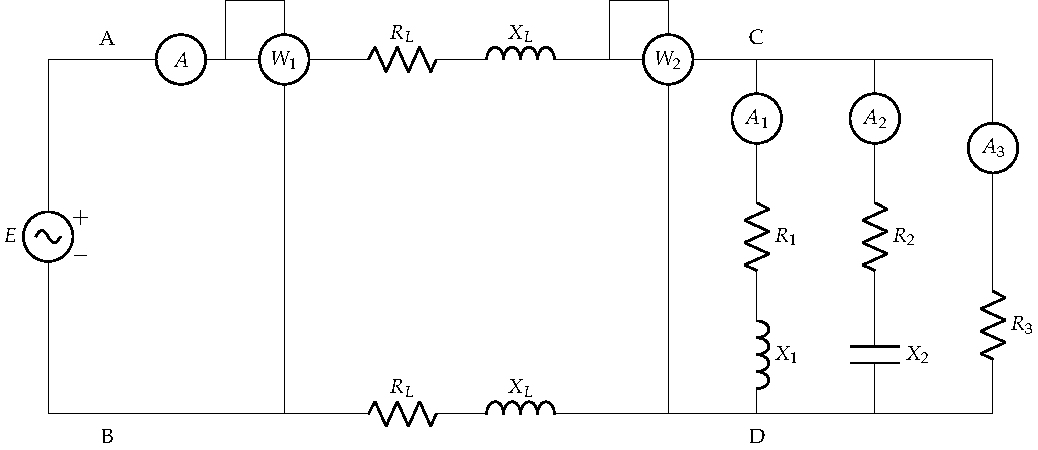
\includegraphics[width=0.85\linewidth]{figuras/BT2_08.pdf}
\end{center}

Sabiendo que $U_{CD} = \qty{200}{\volt}$ se debe calcular:
\begin{itemize}
\item Intensidades de corriente $I$, $I_1$, $I_2$ e $I_3$ {en forma
    fasorial}, tomando $U_{CD}$ como referencia de fase
\item Lectura de los vatímetros $W_1$ y $W_2$
\end{itemize}

\subsection*{Solución}

Se dice que se tome como referencia de fase el fasor
$\overline{U_{CD}}$:

  \begin{equation*}
    \overline{U}_{CD} = \qty[parse-numbers=false]{200\phase{0}}{\volt}
  \end{equation*}

  
  Esta tensión está aplicada en tres ramas en paralelo, por lo que podemos calcular las corrientes en esas ramas. En primer lugar, calculamos las impedancias:

\begin{align*}
\overline{Z}_1 &= \qty[parse-numbers=false]{10 + \mathrm{j}}{\ohm}\\
%
\overline{Z}_2 &= \qty[parse-numbers=false]{10 - \mathrm{j}}{\ohm}
\end{align*}

A continuación calculamos las corrientes de rama y la corriente total:
\begin{align*}
\overline{I}_1 &= \frac{\overline{U}_{CD}}{\overline{Z}_1} = \qty[parse-numbers=false]{19.8 - 1.98\mathrm{j}}{\ampere}\\
%
\overline{I}_2 &= \frac{\overline{U}_{CD}}{\overline{Z}_2} = \qty[parse-numbers=false]{19.8 + 1.98\mathrm{j}}{\ampere}\\
%
\overline{I}_3 &= \frac{\overline{U}_{CD}}{R_3} = \qty[parse-numbers=false]{20\phase{\ang{0}}}{\ampere}\\
%
\overline{I} &= \overline{I}_1 + \overline{I}_2 + \overline{I}_3 =  \qty[parse-numbers=false]{59.6\phase{\ang{0}}}{\ampere}\\
\end{align*}

Para obtener la lectura del vatímetro 2 podemos calcular con tensión y corriente:
  \begin{align*}
\overline{S}_2 &= \overline{U}_{CD} \cdot \overline{I}^* = \qty[parse-numbers=false]{11920\phase{\ang{0}}}{VA}\\
%
W_2 &= \mathrm{Re}\{\overline{S}_2\} = \qty{11920}{\watt}
\end{align*}

O mediante teorema de Boucherot:
\begin{align*}
  P_1 = I_1^2 \cdot R_1 &= \qty{3959.6}{\watt}\\
  P_2 = I_2^2 \cdot R_2 &= \qty{3959.6}{\watt}\\
  P_3 = I_3^2 \cdot R_3 &= \qty{4000}{\watt}\\
  W_2 = P = P_1 + P_2 + P_3 &= \qty{11919.2}{\watt}
\end{align*}

Para el vatímetro 1 hay que tener en cuenta la potencia disipada en la línea, y aplicar nuevamente el teorema de Boucherot.
\begin{align*}
P_l &= 2 \cdot I^2 \cdot R_L = \qty{7105.3}{\watt}\\
W_1 &= W_2 + P_l = \qty{19026}{\watt}
\end{align*}


%%%%%%%%%%%%%%%%%%%%%%%%%%%%%%%%%%%%%%%%%%%%%%%%%%%%%%%%%%%%%%%%%%

\section{Enunciado}
En el circuito los amperímetros $A_1$ y $A_2$ marcan $\qty{4.5}{\ampere}$ y $\qty{6}{\ampere}$, respectivamente; el voltímetro, $\qty{150}{\volt}$ y el
vatímetro $\qty{900}{\watt}$.

Sabiendo que la frecuencia del generador es de $\qty{250}{\hertz}$ y el f.d.p. de la impedancia $Z$ es de 0.8 en retraso, calcula:

\begin{itemize}
\item Valores de R, C y Z en forma compleja
\item La tensión del generador
\item Triángulo de potencias totales.
\end{itemize}

\begin{center}
  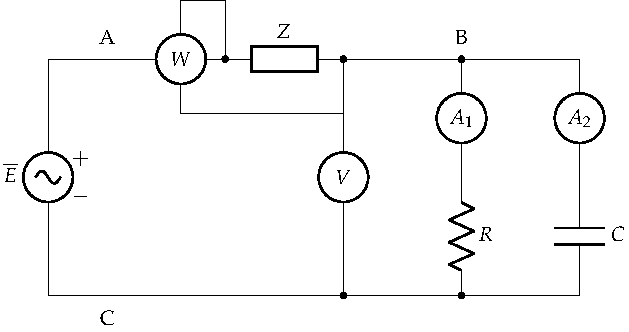
\includegraphics[width=0.45\linewidth]{figuras/BT2_09.pdf}
\end{center}


\subsection*{Solución}
\begin{enumerate}
\item Valores de R, C y Z en forma compleja.
  
\begin{equation*}
    R = \frac{U_{BC}}{A_1} = \frac{150}{4.5} = \qty{33.3}{\ohm}
  \end{equation*}

  \begin{equation*}
    X_c = \frac{U_{BC}}{A_2} = \frac{150}{6} = \qty{25}{\ohm}
  \end{equation*}

  \begin{equation*}
    C = \frac{1}{X_c\omega} = \frac{1}{25 \cdot 2 \pi \cdot 250} = \qty{25.46}{\micro\farad}
  \end{equation*}

  Tomando $\overline{U}_{BC}$ como origen de fases, $\overline{U}_{BC} = \qty[parse-numbers=false]{150\phase{0}}{\volt}$, obtenemos:

  \begin{align*}
    \overline{I}_1 &= \qty[parse-numbers=false]{4.5\phase{0}}{\ampere}\\
    \overline{I}_2 &= \qty[parse-numbers=false]{6\phase{\pi/2}}{\ampere}
  \end{align*}

  Por tanto,
  \[
    \overline{I} = \overline{I}_1 + \overline{I}_2 = \qty[parse-numbers=false]{4.5+6j}{\ampere} = \qty[parse-numbers=false]{7.5\phase{\ang{53.13}}}{\ampere}
  \]
  El vatímetro está midiendo $P_Z = U_Z \cdot I \cos \theta_Z$, y por tanto:

  \[
    U_Z = \frac{900}{7.5 \cdot 0.8} = \qty{150}{\volt}
  \]

  \[
    Z = \frac{U_Z}{I} = \qty{20}{\ohm}
  \]

    También puede obtenerse este resultado calculando primero la parte resistiva de la impedancia:

  \[
    R_Z = \frac{P_Z}{I^2} = \qty{16}{\ohm}
  \]
  y a continuación el módulo teniendo en cuenta que $R = Z \cdot \cos \theta$:

  \[
    Z = \frac{R}{\cos \theta} = \frac{16}{0.8} = \qty{20}{\ohm}
  \]

  Con su factor de potencia obtenemos el ángulo (teniendo en cuenta que es inductiva al ser en retraso), $\theta_Z = \arccos(0.8) = \ang{36.87}$:

  \[
    \overline{Z} = 16 + 12j  = \qty[parse-numbers=false]{20\phase{\ang{36.87}}}{\ohm}
  \]

  
\item Tensión del generador.

  \[
    \overline{U}_{AC} = \overline{U}_{AB} + \overline{U}_{BC}
  \]

  \[
    \overline{U}_{AB} = \overline{Z} \cdot \overline{I} = \qty[parse-numbers=false]{150\phase{\ang{90}}}{\volt}
  \]

  \[
    \overline{U}_{AC} = 150 + 150j = \qty[parse-numbers=false]{150\sqrt{2}\phase{\ang{45}}}{\volt}
  \]

\item Triángulo de potencias totales en forma compleja.

  Podemos calcular a partir de la tensión y la corriente:


  \begin{align*}
    \overline{S}_T &= \overline{U}_{AC} \overline{I}^* =\\
                   &= 150\sqrt{2}\phase{\ang{45}} \cdot 7.5\phase{\ang{-53.13}} =\\
                   &= \qty[parse-numbers=false]{1591\phase{\ang{-8.13}}}{\voltampere}=\\
                   &= \qty[parse-numbers=false]{1575 - j225}{\voltampere}
  \end{align*}
  
  o mediante el teorema de Boucherot:
  \begin{align*}
    P_Z &= \qty{900}{\watt}\\
    P_R = 4.5^2 \cdot 33.3 &= \qty{675}{\watt}\\
    P = P_Z + P_R &= \qty{1575}{\watt}
  \end{align*}

  \begin{align*}
    Q_Z = 7.5^2 \cdot 12 &= \qty{675}{\voltampere_r}\\
    Q_c = - 6^2 \cdot 25 &= \qty{-900}{\voltampere_r}\\
    Q = Q_Z + Q_c &= \qty{-225}{\voltampere_r}
  \end{align*}
  Por tanto:

  \[
    \overline{S} = P + jQ = \qty[parse-numbers=false]{1575 - j225}{\voltampere}
  \]
  
\end{enumerate}

%%%%%%%%%%%%%%%%%%%%%%%%%%%%%%%%%%%%%%%%%%%%%%%%%%%%%%%%%%%%%%%%%%

\section{Enunciado}

En el circuito de la figura, determinar las lecturas de los aparatos de medida y el balance de potencias activas y reactivas, así como el triángulo global de potencias.\\
Datos: $e(t)=100\sqrt{2}\cos(\omega\,t)$; $R_1=2\Omega$;
$R_2=4\Omega$; $\omega\,L_1=3\Omega$; $\omega L_2=4\Omega$.

\begin{center}
  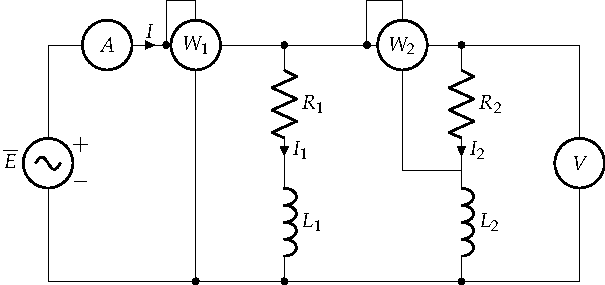
\includegraphics{figuras/BT2_11.pdf}
\end{center}

\subsection*{Solución}

El voltímetro $V$ mide la tensión eficaz de la fuente, por lo que:
\begin{equation*}
  V=\qty{100}{\volt}
\end{equation*}

Las impedancias de las dos ramas son:

\begin{align*}
  \overline{Z}_1 &= R_1 + jX_1 = \qty[parse-numbers=false]{2 + j3}{\ohm}\\
  \overline{Z}_2 &= R_2 + jX_2 = \qty[parse-numbers=false]{4 + j4}{\ohm}
\end{align*}

Calculamos el valor eficaz de las corrientes de rama:

\begin{align*}
  I_1 &= E/Z_1 = \qty{27.74}{\ampere}\\
  I_2 &= E/Z_2 = \qty{17.68}{\ampere}\\
\end{align*}

El vatímetro $W_2$ mide la potencia de $R_2$:
\begin{equation*}
  W_2=R_2 \cdot I_2^2= \qty{1250.33}{\watt}
\end{equation*}

El vatímetro $W_1$ mide la potencia total del circuito:
\begin{equation*}
  W_1= P_{R2} + P_{R1} = R_2 \cdot I_2^2 + R_1 \cdot I_1^2 = \qty{2789.35}{\watt}
\end{equation*}

Por otra parte, las potencias reactivas de las bobinas son:
\begin{align*}
  Q_{L1} &= X_1 \cdot I_1^2 = \qty{2308.52}{\voltampere}_r\\
  Q_{L2} &= X_2 \cdot I_2^2 = \qty{1250.33}{\voltampere}_r
\end{align*}

Por tanto, la potencia reactiva total es $Q = \qty{3558.82}{\voltampere}_r$. Con el valor de la potencia activa podemos obtener la potencia aparente total:

\begin{equation*}
  S = \sqrt{P^2 + Q^2} = \qty{4521.69}{\voltampere}
\end{equation*}

Y, finalmente, la corriente medida por el amperímetro:

\begin{equation*}
  I = S/V = \qty{45.2}{\ampere}
\end{equation*}

%%%%%%%%%%%%%%%%%%%%%%%%%%%%%%%%%%%%%%%%%%%%%%%%%%%%%%%%%%%%%%%%%%

\section{Enunciado}
El circuito de la figura tiene carácter inductivo.  La impedancia de
linea es $Z=\qty[parse-numbers=false]{10\sqrt{2}}{\ohm}$ con
f.d.p. $\sqrt{2}/2$ en retraso. Tómese como referencia de fases la
intensidad total, $I$

Se debe calcular:

\begin{enumerate}

\item \textbf Potencia activa y reactiva consumida por $Z$.

\item  \textbf Expresiones complejas de las intensidades medidas por los
  amperímetros, $I$, $I_1$, $I_2$ e $I_3$. 

\item  \textbf Expresiones complejas de las tensiones $U_{AB}$, $U_{AC}$ y
  $U_{CB}$.

\item  \textbf Valores de $R_1$, $X_1$, $R_2$, $R_3$ y $X_3$.

\end{enumerate}

Datos: $A = \qty[parse-numbers = false]{5\sqrt{5}}{\ampere}$; $A_1 = \qty[parse-numbers = false]{5\sqrt{2}}{\ampere}$; $A_2 = \qty{5}{\ampere}$;  $A_3 = \qty[parse-numbers = false]{\sqrt{10}}{\ampere}$;  $U_{AB} = \qty{247}{\volt}$;  $W_1 = \qty{2350}{\watt}$;
$R_1 = R_3$.

\begin{center}
  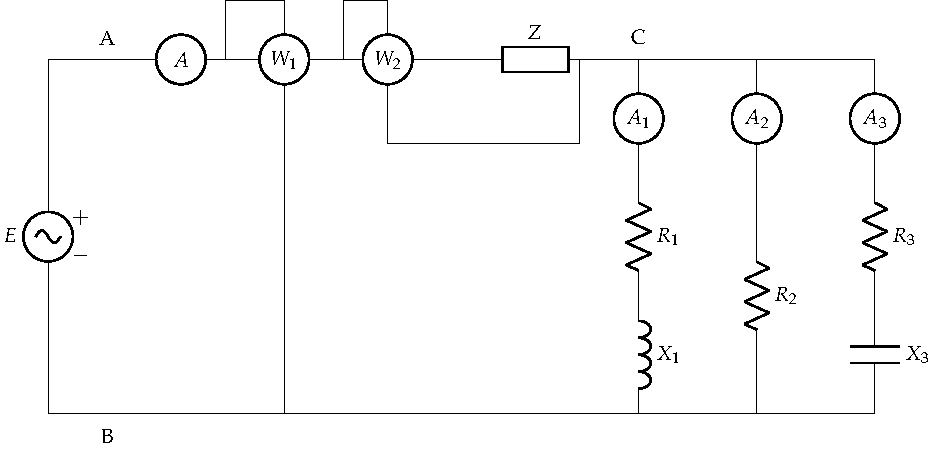
\includegraphics[width=0.8\linewidth]{figuras/BT2_17.pdf}
\end{center}


\subsection*{Solución}

Dado que disponemos de la potencia y corriente total y la tensión a
la entrada, podemos calcular el factor de potencia del circuito:

\[
\cos \phi = \frac{P_1}{U_{AB} I} = 0,851
\]

Teniendo en cuenta que la corriente total es la referencia de fases, 

\[
\overline{U}_{AB} = \qty[parse-numbers=false]{247 \phase{\ang{31.68}}}{\V}
\]

También podemos calcular la potencia reactiva del circuito
(positiva dado que el circuito es inductivo):
\[
Q = P \tan \phi = \qty{1450.4}{VA}r
\]


En cuanto a la impedancia $Z$, sabemos que la tensión en sus bornes
es:

\[
\overline{U}_{AC} = \overline{I} \cdot \overline{Z} =
5\sqrt{5}\phase{\ang{0}} \cdot 10\sqrt{2}\phase{\ang{45}} = \qty[parse-numbers=false]{50\sqrt{10}\phase{\ang{45}}}{\V}
\]

Se cumple que $\overline{U}_{AB} = \overline{U}_{AC} +
\overline{U}_{CB}$, y por tanto:

\[
\overline{U}_{CB} = \qty[parse-numbers=false]{100\phase{\ang{10.3}}}{\V}
\]

Por otra parte, podemos descomponer esta impedancia en:
\begin{align*}
  R &= Z \cdot \cos \phi_Z = \qty{10}{\ohm}\\
  X &= Z \cdot \sin \phi_Z = \qty{10}{\ohm}
\end{align*}

y por tanto,

\begin{align*}
P_z &= I^2 \cdot R_z = \qty{1250}{\watt}\\
Q_z &= I^2 \cdot X_z = \qty{1250}{VA}r
\end{align*}

Aplicando el teorema de Boucherot podemos calcular la potencia activa
y la potencia reactiva del circuito paralelo:

\begin{align*}
P_{CB} &= P - P_z = \qty{1100}{\watt}\\
Q_{CB} &= Q - Q_z = \qty{200}{VA}r\\
\overline{S}_{CB} &= P_{CB} + i Q_{CB} = \qty[parse-numbers=false]{1118.03\phase{\ang{10.3}}}{VA}
\end{align*}

Podemos comprobar que estos resultados son coherentes con los
resultados anteriores usando $\overline{S}_{CB} = \overline{U}_{CB}
\cdot \overline{I}^*$.


Ahora podemos obtener $R_2$, $Z_1$ y $Z_3$:

\begin{align*}
  R_2 &= \frac{U_{CB}}{I_2} = \qty{20}{\ohm}\\
  Z_1 &= \frac{U_{CB}}{I_1} = \qty[parse-numbers=false]{10\sqrt{2}}{\ohm}\\
  Z_3 &= \frac{U_{CB}}{I_3} = \qty[parse-numbers=false]{10\sqrt{10}}{\ohm}
\end{align*}

Con los valores de $Z_1$ y $Z_3$ podemos escribir:

\begin{align*}
  Z_1^2 &= R_1^2 + X_1^2 = 200\\
  Z_3^2 &= R_3^2 + X_3^2 = 1000\\
\end{align*}

Por otra parte, la potencia activa del circuito paralelo es:
\begin{align*}
  P_{CB} &= P_1 + P_2 + P_2 =\qty{1100}{\watt}\\
  P_1 &= I_1^2 \cdot R_1 = 50 \cdot R_1\\
  P_2 &= I_2^2 \cdot R_2 = \qty{500}{\watt}\\
  P_3 &= I_3^2 \cdot R_3 = 10 \cdot R_3
\end{align*}

Por tanto, 
\[
   R_1 = R_3 = \qty{10}{\ohm}              
\]

Con este resultado, teniendo en cuenta el módulo de $Z_1$ y $Z_3$,
podemos calcular las reactancias respectivas.

\begin{align*}
  R_1 &= \qty{10}{\ohm}\\
  X_1 &= \qty{10}{\ohm}\\
  \overline{Z}_1 &= 10 + 10i = \qty[parse-numbers=false]{10\sqrt{2}\phase{\ang{45}}}{\ohm}
\end{align*}

\begin{align*}
  R_3 &= \qty{10}{\ohm}\\
  X_3 &= \qty{30}{\ohm}\\
  \overline{Z}_3 &= 10 - 30i = \qty[parse-numbers=false]{10\sqrt{10}\phase{\ang{-71.56}}}{\ohm}
\end{align*}

Podemos comprobar que estas soluciones concuerdan con la potencia
reactiva de cada impedancia y con la total.

\begin{align*}
  Q_1 &= I_1^2 \cdot X_1 = \qty{500}{VA}r\\
  Q_3 &= - I_3^2 \cdot X_3 = \qty{-300}{VA}r\\
  Q_{CB} &= Q_1 + Q_3 =\qty{200}{VA}r
\end{align*}

Con estos resultados, recordando que  $\overline{U}_{CB} =
100\phase{\ang{10.3}}$ podemos calcular las corrientes en forma
compleja:

\begin{align*}
  \overline{I}_1 &=  \qty[parse-numbers=false]{5\sqrt{2}\phase{\ang{-34.7}}}{\ampere}\\
  \overline{I}_2 &=  \qty[parse-numbers=false]{5\phase{\ang{10.3}}}{\ampere}\\
  \overline{I}_3 &=
  \qty[parse-numbers=false]{\sqrt{10}\phase{\ang{81.9}}}{\ampere}
\end{align*}

Para terminar, podemos comprobar que $\overline{I} = \overline{I_1}
+ \overline{I_2} + \overline{I_3}$.

%%%%%%%%%%%%%%%%%%%%%%%%%%%%%%%%%%%%%%%%%%%%%%%%%%%%%%%%%%%%%%%%%%

\section{Enunciado}

La potencia reactiva del circuito de la figura es $\qty{80}{\voltampere_r}$ de tipo capacitivo. La tensión en la impedancia Z está en fase con la intensidad $I_1$ y las lecturas de los aparatos son $A = \qty{4}{\ampere}$, $V = \qty{50}{\volt}$, $W = \qty{200}{\watt}$. Sabiendo que $R_1 = \qty{10}{\ohm}$ y $X_2 = \qty{50}{\ohm}$, calcula:

\begin{enumerate}
\item Las corrientes $I_1$, $I_2$, $I_3$ en forma fasorial.
\item Las reactancias $X_1$, $X_3$, y la impedancia $\overline{Z}$.
\item La fuerza electromotriz $\overline{\epsilon}$.
\end{enumerate}
\begin{center}
  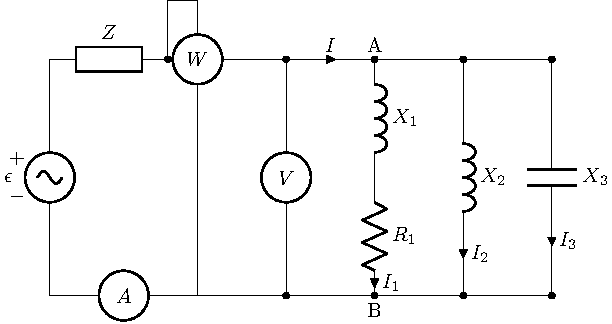
\includegraphics{figuras/BT2_circuitoCapacitivo}
\end{center}

\subsection*{Solución}


El vatímetro está midiendo la potencia activa del circuito paralelo conectado entre A y B. El único elemento que consume potencia activa en ese circuito es la resistencia $R_1$. Por tanto,

\[
  P_{R1} = 200 = I_1^2 R_1 \rightarrow I_1 = \qty[parse-numbers=false]{2\sqrt{5}}{\ampere}
\]

Dado que conocemos la tensión entre A y B, podemos determinar la impedancia de la rama 1:

\[
  Z_1 = \frac{V_{AB}}{I_1} = \qty[parse-numbers=false]{5\sqrt{5}}{\ohm}
\]
y, por tanto, obtenemos $X_1$:

\[
  Z_1 = \sqrt{R_1^2 + X_1^2} \rightarrow X_1 = \qty{5}{\ohm}
\]

\[
  \overline{Z}_1 = 10 + j5 = \qty[parse-numbers=false]{5\sqrt{5}\phase{\ang{26.56}}}{\ohm} 
\]

Para obtener las corrientes en forma fasorial necesitamos una referencia de fases, y será la tensión $U_{AB}$:

\[
  \overline{U}_{AB} = \qty[parse-numbers=false]{50\phase{\ang{0}}}{\volt}
\]

Además, del circuito AB conocemos la tensión, la corriente y la potencia, luego podemos obtener su factor de potencia:

\[
  \cos\theta_{AB} = \frac{P_{AB}}{I \cdot U_{AB}} = 1
\]

Por tanto,

\[
  \overline{I} = \qty[parse-numbers=false]{4\phase{\ang{0}}}{\ampere}
\]


Con $\overline{U}_{AB}$ podemos calcular el ángulo de la corriente $I_1$:

\[
  \overline{I}_1 = \frac{\overline{U}_{AB}}{\overline{Z}_1} = \qty[parse-numbers=false]{2\sqrt{5}\phase{\ang{-26.56}}}{\ampere} 
\]

De la misma forma podemos calcular la corriente $I_2$:
\[
  \overline{I}_2 = \frac{\overline{U}_{AB}}{jX_2} = \qty[parse-numbers=false]{1\phase{\ang{-90}}}{\ampere} 
\]
  
Mediante la LKC podemos obtener la corriente en la rama 3:

\[
  \overline{I} = \overline{I}_1 + \overline{I}_2 + \overline{I}_3 \rightarrow \overline{I}_3 = \qty[parse-numbers=false]{3\phase{\pi/2}}{\ampere}
\]

Aplicamos el teorema de Boucherot para obtener la reactancia de la rama 3, teniendo que en cuenta que $\cos(\theta_{AB}) = 1 \rightarrow Q_{AB} = 0$:

\begin{align*}
  Q &= Q_1 + Q_2 + Q_3 = 0\\
  Q_1 &= I_1^2 X_1 = \qty{100}{\voltampere_r}\\
  Q_2 &= I_2^2 X_2 = \qty{50}{\voltampere_r}\\
  Q_3 &= - I_3^2 X_3
\end{align*}

Por tanto,

\[
   Q_3 = -\qty{150}{\voltampere_r} \rightarrow X_3 = \qty[parse-numbers=false]{\frac{50}{3}}{\ohm}
\]

Para determinar $\overline{Z}$ tenemos en cuenta que la potencia reactiva total es $\qty{80}{\voltampere_r}$ de tipo capacitivo y que $Q_{AB} = \qty{0}{\voltampere}_r$:

\[
  Q = Q_Z + Q_{AB} \rightarrow Q_Z = -\qty{80}{\voltampere_r} 
\]

Por tanto:

\[
  X_Z = \frac{|Q_Z|}{I^2} = \qty{5}{\ohm}
\]

Por otra parte, el enunciado indica que la tensión en esta impedancia está en fase con la intensidad $I_1$. Por tanto, $\theta_{VZ} = \ang{-26.56}$, y $\theta_Z = \theta_{VZ} - \theta_{I} = \ang{-25.56}$. Con este ángulo podemos calcular el valor de la resistencia:

\[
  R_Z = \frac{X_Z}{|\tan\theta_Z|} = \qty{10}{\ohm}
\]

\[
  \overline{Z} =  \qty[parse-numbers=false]{10 - j5}{\ohm}
\]

Finalmente, para calcular la fuerza electromotriz podemos hacerlo de dos formas, mediante potencias o mediante tensiones:

Mediante el teorema de Boucherot calculamos la potencia activa:
\[
P = P_Z + P_{AB} = I^2 R_Z + 200 = \qty{360}{\watt}
\]
Y con la potencia reactiva $Q$ obtenemos la potencia aparente:

\[
  \overline{S} = P + jQ = \qty[parse-numbers=false]{360 -j80}{\voltampere}
\]
y la tensión:

\[
  \overline{\epsilon} = \frac{\overline{S}}{\overline{I}^*} = 90 - j20 = \qty[parse-numbers=false]{10\sqrt{85}\phase{\ang{-12.53}}}{\volt}
\]

Podemos llegar a este mismo resultado con un balance de tensiones:

\[
  \overline{\epsilon} = \overline{U}_Z + \overline{U}_{AB} = \overline{Z} \cdot \overline{I} + \overline{V}_{AB}
\]
%%%%%%%%%%%%%%%%%%%%%%%%%%%%%%%%%%%%%%%%%%%%%%%%%%%%%%%%%%%%%%%%%%
\section{Enunciado}
Un motor monofásico de $S = \qty{10}{\kilo\voltampere}$ y $fdp = 0.8$ está alimentado por una fuente de $\qty{230}{\volt}$ a $f = \qty{50}{\hertz}$. 
Calcula:
\begin{enumerate}
\item El valor eficaz de la corriente absorbida por el motor.
\item La potencia aparente del generador.
\item La capacidad del condensador necesario para compensar el factor de potencia a la unidad.
\item El valor eficaz de la corriente absorbida por el conjunto condensador-motor. 
\item La potencia aparente del generador necesario una vez conectado el condensador del tercer apartado.
\item Compara de forma razonada los resultados de los apartados 4 y 5 con los valores calculados en los apartados 1 y 2.
\end{enumerate}
\begin{enumerate}

\subsection*{Solución}

\item El valor eficaz de la corriente absorbida por el motor.


  \begin{align*}
  \overline{S}_m &= \overline{U} \cdot \overline{I}^*\\
%
  I &= \frac{\num{10000}}{230} = \qty{43.5}{\ampere}
\end{align*}

\item La potencia aparente del generador.
Suponemos línea ideal (sin perdidas):
\[
  S_g = S_m = \qty{10}{\kilo\voltampere} 
\]

\item La capacidad del condensador necesario para compensar el factor de potencia a la unidad.
\begin{align*}
Q_m &= S \cdot \sin(\theta_m) = \qty{6}{\kilo\voltampere_r}\\
Q_c &= Q_m\\
C &= \frac{Q_m}{\omega \cdot V^2} = \qty{361}{\micro\farad}
\end{align*}

\item El valor eficaz de la corriente absorbida por el conjunto condensador-motor. 
\begin{align*}
Q' &= \qty{0}{\voltampere_r}\\
S' &= P_m = \qty{8}{\kilo\voltampere}\\
I' &= \frac{S'}{V} = \qty{34.8}{\ampere}
\end{align*}

\item La potencia aparente del generador necesario una vez conectado el condensador del tercer apartado.
\begin{align*}
S'_g &= S' = \qty{8}{\kilo\voltampere}\\
\end{align*}

\item Compara de forma razonada los resultados de los apartados 4 y 5 con los valores calculados en los apartados 1 y 2.

  La compensación de reactiva mediante la inserción del condensador ha reducido la corriente que circula por la línea y la potencia del generador en un 20\%.

\end{enumerate}

%%%%%%%%%%%%%%%%%%%%%%%%%%%%%%%%%%%%%%%%%%%%%%%%%%%%%%%%%%%%%%%%%% 

\section{Enunciado}
                                              
Un generador de corriente alterna monofásica ($f=50$ Hz) alimenta a dos
cargas a través de una línea de cobre. Esta línea, de resistividad
$\rho=21$ m$\Omega$ mm$^2$/m, tiene una longitud de 100 m y una sección
de 16 mm$^2$. Las dos cargas, cuya tensión de alimentación es de 230 V,
son dos motores, uno con potencia de 7 kW y f.d.p. de $0.65$, y otro con
una potencia de 5 kW y f.d.p. de $0.85$. Con esta información, se pide
calcular:
\begin{itemize}
\item Triángulo de potencias de cada carga y del conjunto de ambas
\item Valor eficaz de las corrientes en cada carga y de la corriente
  total
\item Triángulo de potencias del generador
\item Valor eficaz de la tensión en bornes del generador
\item Capacidad del condensador a instalar en bornes de las cargas para
  mejorar el factor de potencia a $0.95$
\item Valor eficaz de la corriente entregada por el generador una vez
  instalado el condensador
\item Triángulo de potencias del generador una vez instalado el
  condensador
\end{itemize}

\subsection*{Solución}

Las potencias del motor 1 son:
\begin{align*}
  P_1&=7000W\\ Q_1&=P_1\,\tan(\phi_1)=7000\cdot
                    \tan(\arccos(0.65))=8183.91VAr\\
  S_1&=\dfrac{P_1}{\cos(\phi_1)}=\dfrac{7000}{0.65}=10769.23VA
\end{align*}

y las del motor 2:
\begin{align*}
  P_2&=5000W\\ Q_2&=P_5\,\tan(\phi_2)=5000\cdot
                    \tan(\arccos(0.85))=3098.72VAr\\
  S_2&=\dfrac{P_2}{\cos(\phi_2)}=\dfrac{5000}{0.85}=5882.53VA
\end{align*}

Por el T. Boucherot, la potencia total de las cargas es:

\begin{align*}
  P_T&=P_1+P_2 = 12000W\\
  Q_T&=Q_1+Q_2 = 11282.63VAr\\
  S_T&=\sqrt{P_T^2+Q_T^2}=16471.12VA
\end{align*}

por lo que la instalación conjunta tiene un f.d.p. de:
\begin{equation*}
  f.d.p._T=\dfrac{P_T}{S_T}=\dfrac{12000}{16471.12}=0.7285
\end{equation*}

Por definición de potencia activa, se obtienen los valores eficaces de
las corrientes:
\begin{align*}
  I_1&=\dfrac{P_1}{U\,\cos(\phi_1)}=\dfrac{7000}{230\cdot
       0.65}=46.82\,A\\
  I_2&=\dfrac{P_2}{U\,\cos(\phi_2)}=\dfrac{5000}{230\cdot
       0.85}=25.58\,A\\
  I_T&=\dfrac{P_T}{U\,\cos(\phi_T)}=\dfrac{12000}{230\cdot
       0.7285}=71.62\,A
\end{align*}

La resistencia de cada conductor de la línea es:
\begin{equation*}
  R_l=\rho\,\dfrac{L}{S}=\dfrac{21}{1000}\cdot
  \dfrac{100}{16}=0.13\Omega
\end{equation*}

Así, la potencia perdida en la línea:
\begin{equation*}
  P_L= 2 \cdot R_L \cdot I^2=1346.2W
\end{equation*}

y el triángulo de potencias del generador, por el T. Boucherot:
\begin{align*}
  P_g&=P_L+P_T= 13346.23 W\\ Q_g&=Q_T=11282.63 VAr\\
  S_g&=\sqrt{P_g^2+Q_g^2}=17476.26 VA
\end{align*} por lo que
la tensión a la salida del generador es:
\begin{equation*}
  U_g=\dfrac{S_g}{I}=244.4 V
\end{equation*}

Para mejorar el factor de potencia, se sabe que la potencia reactiva
inicial es 11282.63 VAr. Puesto que se quiere un f.d.p.' de $0.95$, la
potencia reactiva final:
\begin{equation*}
  Q_T'=P_T\,\tan(\phi')=12000\cdot \tan(\arccos(0.95))=3944.21 VAr
\end{equation*} siendo
la potencia reactiva restante la generada por la batería de
condensadores ($Q_C=Q_T'-Q_T=3944.21-11282.63=-7338.42$ VAr). Por
tanto, la capacidad del condensador:
\begin{equation*}
  Q_c=X_c\,I^2=\dfrac{U^2}{X_c}\Rightarrow
  C=\dfrac{Q}{\omega\,U^2}=\dfrac{7338.42}{2\cdot\pi\cdot 50\cdot
    230^2}=441.57 \mu F
\end{equation*} A este
mismo resultado se llegaría a partir de la fórmula:
\begin{equation*}
  C=\frac{P_T \left[\tan (\phi) - \tan (\phi')\right]}{\omega
    U^2}=\dfrac{12000\left[\tan (\arccos(0.7285)) - \tan
      (\arccos(0.95))\right]}{2\cdot\pi\cdot 50\cdot 230^2}=441.66 \mu F
\end{equation*}

Una vez instalado el condensador, la potencia aparente es:
\begin{equation*}
  S_T'=\sqrt{P_T^2+Q_T'^2}=\sqrt{12000^2+3944.21^2}=12631.58\,VA
\end{equation*} siendo
la corriente total en las cargas (entregada por el generador):
\begin{equation*}
  I'=\dfrac{S'}{U}=\dfrac{12631.58}{230}=54.92 A
\end{equation*} Con esta
corriente, la potencia perdida en la línea:
\begin{equation*}
  P_L'=2 \cdot R_L \cdot I'^2= 791.76W
\end{equation*} y el
triángulo de potencias del generador, por el T. Boucherot:
\begin{align*}
  P_g'&=P_L+P_T=12791.75 W\\ Q_g'&=Q_T'=3944.21 VAr\\
  S_g'&=\sqrt{P_g'^2+Q_g'^2}=13386.02 VA
\end{align*}

%%%%%%%%%%%%%%%%%%%%%%%%%%%%%%%%%%%%%%%%%%%%%%%%%%%%%%%%%%%%%%%%%%
\section{Enunciado}
Un generador de corriente alterna monofásica ($f = \qty{50}{\hertz}$) alimenta
a dos cargas a través de una línea de cobre. Esta línea, de
resistividad $\rho = \qty{0.017}{\ohm\per\milli\meter\squared\per\meter}$, tiene una longitud de
\qty{40}{\meter} y una sección de \qty{6}{\milli\meter\squared}. Las dos cargas, cuya tensión de
alimentación es de \qty{200}{\volt}, son:
\begin{enumerate}
\item Un motor de \qty{7}{\kilo\watt} con f.d.p. {0,7}.
\item Un grupo de lámparas fluorescentes con potencia total \qty{200}{\watt} y
  f.d.p. {0,5}.
\end{enumerate}
Se pide:
\begin{itemize}
\item Esquema del circuito señalando adecuadamente los elementos,
  corrientes y tensiones
\item Potencias activa, reactiva y aparente de cada carga
\item Valor eficaz de las corrientes en cada carga, y de la corriente
  total
\item Potencia activa y reactiva entregada por el generador
\item Valor eficaz de la tensión en bornes del generador
\item Capacidad necesaria a instalar en bornes de las cargas para
  mejorar el factor de potencia de las mismas a la unidad
\item Valor eficaz de la tensión en bornes del generador, y potencia
  aparente entregada por el mismo una vez instalada la capacidad
  determinada en el apartado anterior
\end{itemize}

\subsection*{Solución}

\begin{enumerate}
  
\item El esquema del circuito es el mostrado en la figura.

\begin{center}
  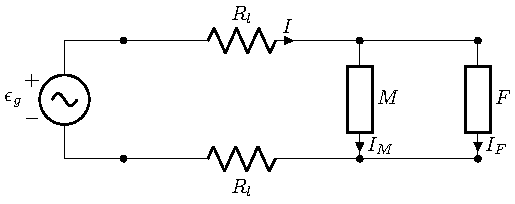
\includegraphics{figuras/circuito_cargas.pdf}
\end{center}
  
\item Potencias activa, reactiva y aparente de cada carga.

\begin{align*}
  P_M &= \qty{7000}{\watt}\\
  Q_M &= \qty{7141.4}{VA}_r\\
  S_M &= \qty{10000}{VA}\\
  P_F &= \qty{200}{\watt}\\
  Q_F &= \qty{346.4}{VA}_r\\
  S_F &= \qty{400}{VA}
\end{align*}

\item Valor eficaz de las corrientes en cada carga, y de la corriente
  total.

  \begin{align*}
    I_M &= S_M / V = \qty{50}{\ampere}\\
    I_F &= S_F / V = \qty{2}{\ampere}
  \end{align*}

  Por teorema de Boucherot la potencia total en cargas es:

\begin{align*}
  P_T &= \qty{7200}{\watt}\\
  Q_T &= \qty{7487.8}{VA}_r\\
  S_T &= \qty{10387.9}{VA}
\end{align*}

Y, por tanto, la corriente total es:
\[
  I = S_T / U = \qty{51.9}{\ampere}
\]

\item Potencia activa y reactiva entregada por el generador.
La resistencia de la línea (una resistencia por cada conductor) es:

\[
R_L = \rho L/S = \qty{0.113}{\ohm}
\]

La potencia activa disipada en la línea es:

\[
P_L = 2 \cdot I^2 R_L = \qty{611.48}{\watt}
\]

Por tanto, la potencia entregada por el generador es:

\begin{align*}
P_g &= P_L + P_T = \qty{7811.5}{\watt}\\
Q_g &= Q_T = \qty{7487.8}{VA}_r\\
S_g &= \qty{10820.7}{VA}
\end{align*}

\item Valor eficaz de la tensión en bornes del generador.
\[
U_g = S_g / I = \qty{208.3}{\volt}
\]

\item Capacidad necesaria a instalar en bornes de las cargas para
  mejorar el factor de potencia de las mismas a la unidad.

  \[
C = \frac{Q_t}{\omega V^2} = \qty{595.9}{\micro\farad}
\]


\item Valor eficaz de la tensión en bornes del generador, y potencia
  aparente entregada por el mismo una vez instalada la capacidad
  determinada en el apartado anterior.

  Una vez instalado este condensador, la corriente total en las cargas es:

\[
I' = P_T / V = \qty{36}{\ampere}
\]

La potencia disipada en la línea es ahora:

\[
P'_L = 2 \cdot I'^2 R_L = \qty{293.8}{\watt} 
\]

Y la potencia entregada por el generador es:
\begin{align*}
P'_g &= \qty{7493.8}{\watt}\\
Q'_g &= \qty{0}{VA}_r\\
S'_g &= \qty{7493.8}{VA}
\end{align*}

Por tanto, la tensión en bornes del generador es:

\[
U'_g = S'_g / I' = \qty{208.2}{\volt}
\]

\end{enumerate}
%%%%%%%%%%%%%%%%%%%%%%%%%%%%%%%%%%%%%%%%%%%%%%%%%%%%%%%%%%%%%%%%%% 

\section{Enunciado}


Un generador de corriente alterna ($f = \SI{50}{\hertz}$) alimenta una instalación eléctrica a través de una línea de cobre ($\rho = \SI{0.017}{\ohm\milli\meter\squared\per\meter}$) de $\SI{25}{\milli\meter\squared}$ de sección. La instalación eléctrica está compuesta por un motor de $S_m = \SI{10}{\kilo\voltampere}$ y $\mathrm{fdp} = 0.8$, una instalación de alumbrado fluorescente de $P_f = \SI{800}{\watt}$ y $\mathrm{fdp} = 0.9$, y diversas cargas electrónicas con una potencia conjunta $P_e = \SI{540}{\watt}$ y $\mathrm{fdp} = 0.5$ en retraso.

Suponiendo que las cargas trabajan a su tensión nominal de $\SI{230}{\volt}$ y que están situadas a $\SI{100}{\meter}$ del generador, calcule:

\begin{enumerate}
\item Triángulo de potencias total de las cargas ($P_T$, $Q_T$, $S_T$) y factor de potencia.
\item Valor eficaz de la corriente que circula por la línea.
\item Potencia disipada en la línea.
\item Triángulo de potencias del generador ($P_g$, $Q_g$, $S_g$) y factor de potencia.
\item Valor eficaz de la tensión de salida del generador.
\item Capacidad del banco de condensadores a instalar en bornes de la carga necesario para reducir la corriente que circula por la línea a un valor de $\SI{45}{\ampere}$.
\end{enumerate}

Independientemente del resultado obtenido, suponga que la capacidad instalada es $C = \SI{172}{\micro\farad}$. En estas condiciones, calcule:
\begin{enumerate}[resume]
\item Potencia aparente de las cargas (incluyendo al banco de condensadores)
\item Valor eficaz de la corriente que circula por la línea y potencia disipada en la misma.
\item Triángulo de potencias del generador y factor de potencia.
\item Tensión de trabajo del generador.
\end{enumerate}

\subsection*{Solución}

\begin{enumerate}
\item Triángulo de potencias total de las cargas ($P_T$, $Q_T$, $S_T$) y factor de potencia.

    Motor:
  \begin{align*}
    P_m &= \SI{8000}{\watt}\\
    Q_m &= \SI{6000}{\voltampere}_r\\
  \end{align*}

  Alumbrado
  \begin{align*}
    P_f &= \SI{800}{\watt}\\
    Q_f &= \SI{387.5}{\voltampere}_r\\
  \end{align*}

  Cargas Electrónicas
  \begin{align*}
    P_e &= \SI{540}{\watt}\\
    Q_e &= \SI{935.3}{\voltampere}_r\\
  \end{align*}

  Total (Teorema de Boucherot)
  \begin{align*}
    P_T &= P_m + P_f + P_e = \SI{9340}{\watt}\\
    Q_T &= Q_m + Q_f + Q_e = \SI{7322.8}{\voltampere}_r\\
  \end{align*}

  Por tanto, $S_T = \SI{11868.4}{\voltampere}$ y
  $\mathrm{fdp}_T = 0.787$.

\item Valor eficaz de la corriente que circula por la línea.
\[
  I = \frac{S_T}{U} = \frac{11868.4}{230} = \SI{51.6}{\ampere}
\]

\item Potencia disipada en la línea.

  \begin{align*}
  R &= \SI{0.068}{\ohm}\\
  P_L &= 2 \cdot I^2 \cdot R = \SI{362.1}{\watt}
  \end{align*}

\item Triángulo de potencias del generador ($P_g$, $Q_g$, $S_g$) y factor de potencia.


  \begin{align*}
    P_g &= P_T + P_L = \SI{9702.1}{\watt}\\
    Q_g &= Q_T = \SI{7322.8}{\voltampere}_r\\
    S_g &= \SI{12155.4}{\voltampere}\\    
    \mathrm{fdp} &= 0.798
  \end{align*}

\item Valor eficaz de la tensión de salida del generador.

  \[
    U_g = \frac{S_g}{I} = \SI{235.6}{\volt}
  \]

\item Capacidad del banco de condensadores a instalar en bornes de la carga necesario para reducir la corriente que circula por la línea a un valor de $\SI{45}{\ampere}$.

  Si la corriente en línea se reduce a $\SI{45}{\ampere}$ la potencia aparente resultante en cargas (incluyendo al condensador) es $S'_T = 230 \cdot 45 = \SI{10350}{\voltampere}$. Por tanto, $Q'_T = \SI{4459.5}{\voltampere}_r$. Así, es necesario instalar un banco de condensadores que aporte $Q_c = Q_T - Q'_T = \SI{2863.3}{\voltampere}_r$.

\[
C = \frac{Q_c}{\omega U^2} = \SI{172.3}{\micro\farad}
\]

  
\end{enumerate}

Independientemente del resultado obtenido, suponga que la capacidad instalada es $C = \SI{172}{\micro\farad}$. En estas condiciones, calcule:
\begin{enumerate}[resume]
\item Potencia aparente de las cargas (incluyendo al banco de condensadores)
\[
S'_T = \sqrt{P^2_T + Q'^2_T} = \SI{10350.1}{\voltampere}
\]

\item Valor eficaz de la corriente que circula por la línea y potencia disipada en la misma.
\[
I' = \frac{S'_T}{U} = \SI{45}{\ampere}
\]

\[
  P'_L = 2 \cdot I'^2 \cdot R = \SI{275.4}{\watt}
\]

\item Triángulo de potencias del generador y factor de potencia.
  \begin{align*}
    P'_g &= P_T + P'_L = \SI{9615.4}{\watt}\\
    Q'_g &= Q'_T = \SI{4459.5}{\voltampere}_r\\
    S'_g &= \SI{10599.2}{\voltampere}\\    
  \end{align*}

\item Tensión de trabajo del generador.
\[
U'_g = \frac{S'_g}{I'} = \SI{235.5}{\volt}
\]
\end{enumerate}

%%%%%%%%%%%%%%%%%%%%%%%%%%%%%%%%%%%%%%%%%%%%%%%%%%%%%%%%%%%%%%%%%% 
\section{Enunciado}

Calcular la corriente $i(t)$ del circuito de la figura.

\begin{center}
  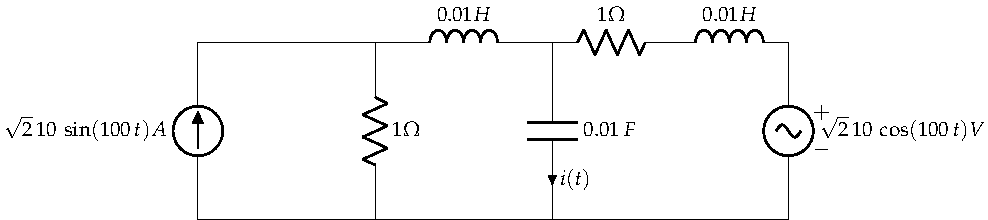
\includegraphics{figuras/BT2_13.pdf}
\end{center}
Datos: $i_g(t) = 10\sqrt{2}\sin(100t)\unit{\ampere}$; $R_1 = R_2 = \qty{1}{\ohm}$; $L_1 = L_2 = \qty{0.01}{\henry}$; $C_1 = \qty{0.01}{\farad}$; $u_g(t) = 10\sqrt{2}\cos(100t)\unit{\volt}$
\subsection*{Solución}

En primer lugar, se deben indicar las dos expresiones de tensión y
corriente en una misma función senoidal. En este caso, se opta por
pasar la corriente a función coseno:

\begin{align*}
  u(t)&=\sqrt{2}\,10\,\cos(100\,t) V\Rightarrow \overline{U}=10\phase{\ang{0}} V\\
  i(t)&=\sqrt{2}\,10\,\cos(100\,t-\frac{\pi}{2}) A\Rightarrow \overline{I}=10\phase{\ang{-90}} A
\end{align*}
Se transforma la fuente de corriente en una fuente de tensión en serie
con la resistencia de 1$\Omega$:
\begin{equation*}
  \overline{U_{Ig}}=\overline{I}\, R_{1}=(10\phase{\ang{-90}})\cdot 1=10\phase{\ang{-90}} V
\end{equation*}
y estableciendo corrientes de malla como se muestra en la siguiente
figura, se puede plantear el sistema de ecuaciones en forma matricial
tras determinar el valor de las imepdancias:
\begin{align*}
  \overline{X_L}&=\mathrm{j}\omega\,L=\mathrm{j} 100\cdot 0.01= \mathrm{j}\Omega\\
  \overline{X_C}&=-\mathrm{j}\dfrac{1}{\omega\,C}=-\mathrm{j} \dfrac{1}{100\cdot 0.01}= -\mathrm{j}\Omega
\end{align*}

\begin{center}
  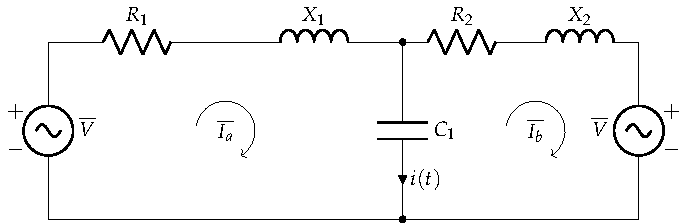
\includegraphics{figuras/BT2_13_mod.pdf}
\end{center}

\begin{equation*}
  \begin{bmatrix}
    1+\mathrm{j}-\mathrm{j} & -(-\mathrm{j})\\
    -(-\mathrm{j}) & 1+\mathrm{j}-\mathrm{j}
  \end{bmatrix}
  \cdot
  \begin{bmatrix}
    \overline{I_a}\\
    \overline{I_b}
  \end{bmatrix}
  =
  \begin{bmatrix}
    10\phase{-90^\circ}\\
    -10\phase{0^\circ}
  \end{bmatrix}
\end{equation*}
cuya solución es:
\begin{align*}
  \overline{I_a}&=0\,A\\
  \overline{I_b}&=-10\,A
\end{align*}
Dado que la corriente $i(t)$ se relaciona con las corrientes de malla
por:
\begin{equation*}
  \overline{I}=\overline{I_a}-\overline{I_b}=0-(-10)=10\,A
\end{equation*}
siendo su expresión temporal:
\begin{equation*}
  i(t)=\sqrt{2}\,10\,\cos(100\,t) A
\end{equation*}

%%%%%%%%%%%%%%%%%%%%%%%%%%%%%%%%%%%%%%%%%%%%%%%%%%%%%%%%%%%%%%%%%%


\section{Enunciado}
Del circuito de la figura, obtener:
\begin{itemize}
\item Expresiones analíticas de las intensidades $i_1(t)$ e $i_2(t)$
\item Potencia disipada por todas las resistencias
\end{itemize}
Datos: $e_g(t)=50\sqrt{2} \cos(1000\,t)$ V; $i_g(t)=10$ A;
$R_1=R_2=2\Omega$; $R_3=7\Omega$; $L_1=L_2=1$ mH; $L_3=2$ mH

\begin{center}
  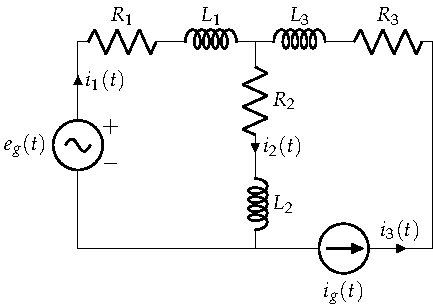
\includegraphics{figuras/BT2_18.pdf}
\end{center}

\subsection*{Solución}

En el circuito hay dos fuentes funcionando a diferentes frecuencias. Por tanto, hay que resolver mediante el principio de superposición.

\textbf{Circuito cuando solo actúa $i_g(t)$}
    
La fuente $e_g(t)$ se cortocircuita y se deja únicamente la fuente
$i_g(t)$. Al ser una fuente de continua, las bobinas se
cortocircuitan. Queda un circuito de dos mallas, donde se sabe que
$I_3'=10$ A. Resolviendo el circuito (por leyes básicas, mallas o
nudos), se obtiene que:
\begin{align*}
  I_1'&=-5\,A\\
  I_2'&=5\,A
\end{align*}
    
Las potencias en este caso:
\begin{align*}
  P_{R1}'&=R_1\,I_1'^2=2\cdot (-5)^2=50\,W\\
  P_{R2}'&=R_2\,I_2'^2=2\cdot 5^2=50\,W\\
  P_{R3}'&=R_3\,I_3'^2=7\cdot 10^2=700\,W\\
\end{align*}
    
\textbf{Circuito cuando solo actúa $e_g(t)$}
    
La fuente $i_g(t)$ queda como un circuito abierto; por tanto, queda un
circuito de una malla e $I_3''=0$ A. Se calculan las reactancias de
las bobinas $L_1$ y $L_2$, sabiendo que $\omega=1000$ rad/s:
\begin{equation*}
  \overline{X_{L1}}=\overline{X_{L2}}=\mathrm{j}\omega L=\mathrm{j}\, 1000\cdot 0.001 = \mathrm{j}\Omega
\end{equation*}
Por la ley de Ohm, tomando valores eficaces, se obtiene el valor de
$\overline{I_1''}=\overline{I_2''}$:
\begin{equation*}
  \overline{I_1''}=\overline{I_2''}=\dfrac{\overline{U}}{\overline{Z_{eq}}}=\dfrac{50\phase{0^\circ}}{2+\mathrm{j}+2+\mathrm{j}}=\underbrace{5\sqrt{5}}_{11.18}\phase{-26.57^\circ} A
\end{equation*}
    
Las potencias en este caso:
\begin{align*}
  P_{R1}''&=R_1\,I_1''^2=2\cdot (5\sqrt{5})^2=250\,W\\
  P_{R2}''&=R_2\,I_2''^2=2\cdot (5\sqrt{5})^2=250\,W\\
  P_{R3}''&=R_3\,I_3''^2=7\cdot 0^2=0\,W\\
\end{align*}
    
\textbf{Expresiones temporales}
    
Por tanto, las expresiones de $i_1(t)$, $i_2(t)$ e $i_3(t)$ son:
\begin{align*}
  i_1(t)&= -5+5\sqrt{10}\cos(1000t-0.46) A \\
  i_2(t)&= 5+5\sqrt{10}\cos(1000t-0.46) A \\
  i_3(t)&= 10 A 
\end{align*}
    
\textbf{Cálculo de $P_T$}
    
La potencia activa total consumida por las resistencias es:
\begin{align*}
  P_T&=R_1\,(I_1'^2+I_1''^2)+R_2\,(I_2'^2+I_2''^2)+R_3\,(I_3'^2+I_3''^2)=\\
     &=2\cdot((-5)^2+(5\sqrt{5})^2)+2\cdot(5^2+(5\sqrt{5})^2)+7\cdot (10^2+0^2)={1300\,W}
\end{align*}
que coincide con el valor obtenido al sumar las potencias de cada
circuito (debido a la ortogonalidad de las señales implicadas):
\begin{equation*}
  P_T=P_{R1}'+P_{R2}'+P_{R3}'+P_{R1}''+P_{R2}''+P_{R3}''=50+50+700+250+250+0=1300\,W
\end{equation*}

%%%%%%%%%%%%%%%%%%%%%%%%%%%%%%%%%%%%%%%%%%%%%%%%%%%%%%%%%%%%%%%%%%

\section{Enunciado}
En el circuito de la figura determina:
\begin{itemize}
\item $u_R(t)$ y $u_L(t)$
\item Balance de potencias
\end{itemize}
Datos:
\begin{equation*}
  e_a(t) = \qty[parse-numbers=false]{3\sqrt{2} \sin(10^3 t)}{\volt}; e_b(t) = \qty[parse-numbers=false]{30\sqrt{2} \sin(10^4 t)}{\volt}; R = \qty{30}{\ohm}; L = \qty{3}{\milli\henry} 
\end{equation*}

\begin{center}
  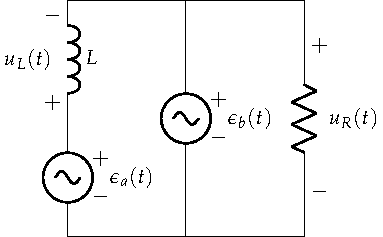
\includegraphics{figuras/superposicion2_ej.pdf}
\end{center}

\subsection*{Solución}

Dado que las fuentes trabajan a frecuencias diferentes, hay que resolver mediante superposición.

Activamos una de las fuentes:
\begin{center}
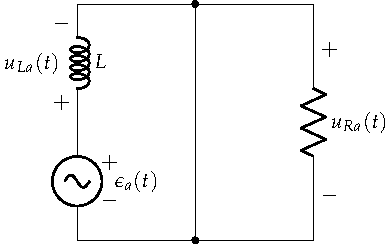
\includegraphics{figuras/superposicion2_A}
\end{center}

La resistencia está cortocircuitada. Por tanto:

\begin{align*}
  u_{Ra}(t) &= \qty{0}{\volt}\\
  u_{La}(t) &= \epsilon_a(t)\\  
\end{align*}

En este circuito la potencia disipada por la resistencia es $P_{Ra} = \qty{0}{\watt}$ y, en consecuencia, la potencia entregada por el generador es $P_{\epsilon_a} = \qty{0}{\watt}$.

Hacemos el análisis con la otra fuente:

\begin{center}
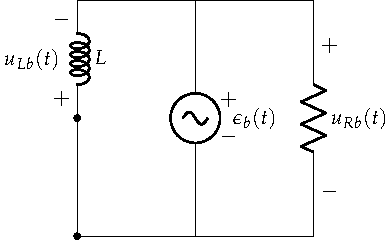
\includegraphics{figuras/superposicion2_B}
\end{center}

En este circuito:

\begin{align*}
  u_{Rb}(t) &= \epsilon_b(t)\\
  u_{Lb}(t) &= -\epsilon_b(t)\\  
\end{align*}

El balance de potencias es:

\begin{equation*}
  P_{Rb} = \frac{\epsilon_b^2}{R_b} = \qty{30}{\watt} = P_{\epsilon_b}\\
\end{equation*}

Por tanto:

\begin{align*}
  u_R(t) &= u_{Ra}(t) + u_{Rb}(t) = 30\sqrt{2}\sin(10^4 t)\\
  u_L(t) &= u_{La}(t) + u_{Lb}(t) = 3\sqrt{2}\sin(10^3 t) - 30\sqrt{2}\sin(10^4 t)\\
\end{align*}

Además, dado que las dos señales de los generadores son ortogonales, podemos sumar las potencias calculadas en cada circuito:

\begin{align*}
  P_R &= P_{Ra} + P_{Rb} = \qty{30}{\watt}\\
  P_\epsilon &= P_{\epsilon_a} + P_{\epsilon_b} = \qty{30}{\watt}\\
\end{align*}

%%%%%%%%%%%%%%%%%%%%%%%%%%%%%%%%%%%%%%%%%%%%%%%%%%%%%%%%%%%%%%%%%%

\section{Enunciado}
El circuito de la figura se encuentra en régimen permanente. Determinar analíticamente la expresión de $i(t)$, así como las potencias entregadas por los generadores y disipadas por las resistencias $R_1$ y $R_2$.

Datos:
\begin{align*}
  e_1(t) = \qty[parse-numbers=false]{50 \sin(1000 t)}{\volt};
  e_2(t) = \qty{30}{\volt};
  R_1 = \qty{6}{\ohm};
  R_2 = \qty{6}{\ohm};
  L = \qty{8}{\milli\henry};
  C = \qty{10}{\micro\farad}
\end{align*}

\begin{center}
  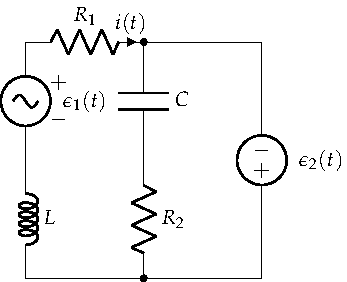
\includegraphics{figuras/superposicion1_ej.pdf}
\end{center}

 \subsection*{Solución}

Aplicamos superposición.

Analizamos con la fuente de corriente alterna:

\begin{center}
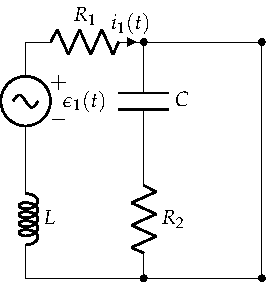
\includegraphics{figuras/superposicion1_AC}
\end{center}

La rama $R_2 - C$ está cortocircuitada y, por tanto, podemos prescindir de ella:

\begin{align*}
  \overline{Z}_1 &= R_1 + jX_L = 6 + 8j\si{\ampere}\\
  \overline{I}_1 &= \overline{\epsilon}_1 / \overline{Z}_1 = 5\sqrt{2}/2\phase{\ang{-53.13}}\si{\ampere}
\end{align*}

En el dominio del tiempo obtenemos:

\begin{equation*}
  i_1(t) = 5\sin(1000t - 0.9273)\si{\ampere}
\end{equation*}

En cuanto al balance de potencias:

\begin{align*}
  P_{R11} &= I_1^2 R_1 = \qty{75}{\watt}\\
  P_{R21} &= \qty{0}{\watt}\\
  P_{\epsilon_1} &= \Re(\overline{\epsilon}_1 \cdot \overline{I}_1^*) = \qty{75}{\watt}
\end{align*}

Analizamos con la fuente de corriente continua:

\begin{center}
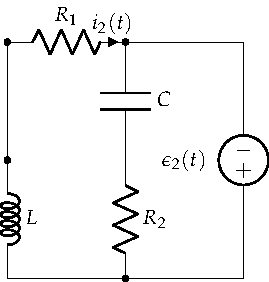
\includegraphics{figuras/superposicion1_DC}
\end{center}

En este circuito sustituimos la bobina por un cortocircuito y el condensador por un circuito abierto. En consecuencia:

\begin{equation*}
  i_2(t) = \epsilon_2(t) / R_1 = \qty{5}{\ampere}
\end{equation*}

En cuanto al balance de potencias:

\begin{align*}
  P_{R12} &= I_2^2 \cdot R_1 = \qty{150}{\watt}\\
  P_{R22} &= \qty{0}{\watt}\\
  P_{\epsilon2} &= \epsilon_2 \cdot I_2 = \qty{150}{\watt}
\end{align*}

Por tanto:

\begin{equation*}
  i(t) = i_1(t) + i_2(t) = 5 + 5\sin(1000t - 0.9273)\si{\ampere}
\end{equation*}

Además, como las señales son ortogonales, podemos hacer el balance de potencias conjunto con los dos circuitos:

\begin{align*}
  P_{R1} &= P_{R11} + P_{R12} = \qty{225}{\watt}\\
  P_{R2} &= P_{R21} + P_{R22} = \qty{0}{\watt}\\
  P_{\epsilon} &= P_{\epsilon1} + P_{\epsilon2} = \qty{225}{\watt}\\
\end{align*}
%%%%%%%%%%%%%%%%%%%%%%%%%%%%%%%%%%%%%%%%%%%%%%%%%%%%%%%%%%%%%%%%%%
\section{Enunciado}
Obtén el generador equivalente de Thévenin del circuito de la figura respecto de A y B.

\begin{center}
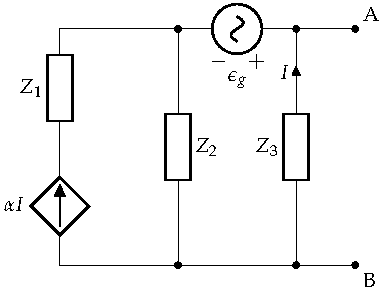
\includegraphics{figuras/Thevenin4}
\end{center}

Datos:
\begin{equation*}
  \overline{\epsilon_g} = \qty[parse-numbers=false]{12 - 16j}{\volt};
  \overline{Z}_1 = \qty[parse-numbers=false]{1 - j}{\ohm};
  \overline{Z}_2 = \qty[parse-numbers=false]{1 + j}{\ohm};
  \overline{Z}_3 = \qty[parse-numbers=false]{5 + 3j}{\ohm}
  \alpha = 2
\end{equation*}


\subsection*{Solución}

Dejamos el circuito en abierto y calculamos la tensión en AB:

\begin{align*}
  \overline{U}_{AB} &= \overline{\epsilon}_g + (1 + \alpha) \overline{I} \cdot \overline{Z}_2\\
  \overline{U}_{AB} &= - \overline{I} \cdot \overline{Z}_3
\end{align*}

Combinando estas ecuaciones obtenemos la tensión:

\begin{equation*}
  \overline{\epsilon}_{th} = \overline{U}_{AB} = \frac{\overline{\epsilon}_g}{1 + (1 + \alpha) \frac{\overline{Z}_2}{\overline{Z}_3}} = 6 - 10j = 11.66\phase{\ang{-59.04}}\si{\volt}
\end{equation*}

Para obtener la impedancia apagamos las fuentes independientes. Como hay fuentes dependientes debemos aplicar una fuente de prueba a la salida del circuito, con fuerza electromotriz $\overline{\epsilon}_0$ y corriente inyectada $\overline{I}_0$.

\begin{minipage}{0.5\linewidth}
  \begin{center}
    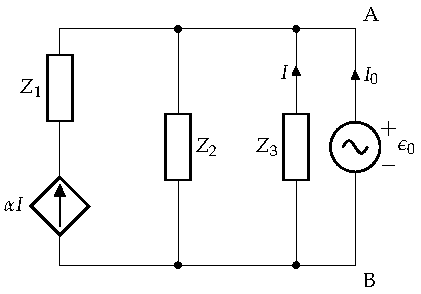
\includegraphics{figuras/Thevenin4_fuenteprueba}
  \end{center}
\end{minipage}
\begin{minipage}{0.5\linewidth}
  \begin{align*}
    \overline{\epsilon}_0 &= [(1 + \alpha) \overline{I} + \overline{I}_0] \cdot \overline{Z}_2\\
    \overline{\epsilon}_0 &= - \overline{I}\cdot \overline{Z}_3
  \end{align*}
\end{minipage}

Combinando ambas expresiones obtenemos:

\begin{equation*}
  \overline{Z}_{th} = \frac{\overline{\epsilon}_0}{\overline{I}_0} = \frac{\overline{Z}_2 \cdot \overline{Z}_3}{(1 + \alpha) \overline{Z}_2 + \overline{Z}_3} = 0.64 + 0.52j\si{\ohm}
\end{equation*}

Para obtener la máxima potencia disponible hay que conectar una impedancia:
\begin{equation*}
\overline{Z}_L = \overline{Z}^*_{th} = 0.64-0.52j\si{\ohm}
\end{equation*}

Esta impedancia disipará una potencia:
\begin{equation*}
P_L = \frac{\epsilon_{th}^2}{4 \cdot R_{th}} = \qty{53.11}{\watt}
\end{equation*}

%%%%%%%%%%%%%%%%%%%%%%%%%%%%%%%%%%%%%%%%%%%%%%%%%%%%%%%%%%%%%%%%%%

\section{Enunciado}

Obtén el generador equivalente de Thévenin del circuito de la figura respecto de A y B. A partir de este generador, calcula la impedancia a colocar en AB para obtener la máxima potencia, calculando esta potencia.

\begin{minipage}{0.5\textwidth}
\begin{center}
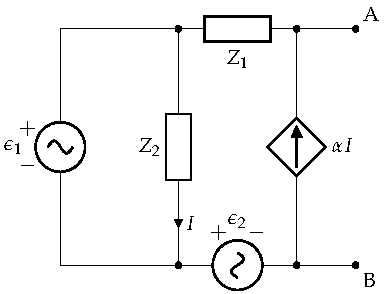
\includegraphics{figuras/Thevenin5}
\end{center}
\end{minipage}
\begin{minipage}{0.5\textwidth}
  \begin{align*}
    \overline{\epsilon_1} &= \SI[parse-numbers=false]{10\phase{0}}{\volt}\\
    \overline{\epsilon_2} &= \SI[parse-numbers=false]{10j}{\volt}\\
    \overline{Z}_1 &= \SI[parse-numbers=false]{4 - 3j}{\ohm}\\
    \overline{Z}_2 &= \SI[parse-numbers=false]{3 + 4j}{\ohm}\\
    \alpha &= 2
  \end{align*}
\end{minipage}
\subsection*{Solución}

La tensión en circuito abierto es:

\begin{equation*}
  \overline{U}_{AB} = \alpha \overline{I} \cdot \overline{Z}_1 + \overline{\epsilon}_1 + \overline{\epsilon}_2
\end{equation*}
siendo $\epsilon_1 = \overline{Z}_2 \cdot \overline{I}$. Por tanto,

\begin{equation*}
  \epsilon_{th}  = \alpha \cdot \overline{\epsilon}_1 \cdot \frac{\overline{Z}_1}{\overline{Z}_2} + \overline{\epsilon}_1 + \overline{\epsilon}_2 = 10 - 10j \si{\volt}
\end{equation*}

Para obtener la impedancia apagamos las fuentes independientes. Al apagar la fuente $\epsilon_1$, la impedancia $Z_2$ queda cortocircuitada y, por tanto, $I = 0$. En consecuencia, la fuente dependiente también queda apagada y obtenemos:

\begin{equation*}
  \overline{Z}_{th} = \overline{Z}_1 = 4 - 3j \si{\ohm}
\end{equation*}

Para obtener la máxima potencia debemos conectar la impedancia:

\begin{equation*}
  \overline{Z}_{L} = \overline{Z}^*_{th} = 4 + 3j \si{\ohm}
\end{equation*}

El balance de potencias es:

\begin{align*}
  P_L &= \frac{\epsilon_{th}^2}{4 \cdot R_{th}} = \SI{12.5}{\watt}\\
  P_{\epsilon} &= 2 \cdot P_L = \SI{25}{\watt} 
\end{align*}
%%%%%%%%%%%%%%%%%%%%%%%%%%%%%%%%%%%%%%%%%%%%%%%%%%%%%%%%%%%%%%%%%%

%%% Local Variables:
%%% mode: latex
%%% TeX-master: "Problemas_TC"
%%% ispell-local-dictionary: "castellano"
%%% End:

